\documentclass[journal]{IEEEtran}

\usepackage{amsmath,amssymb,amsthm}
\usepackage{algorithm}
\usepackage{algpseudocode}
\usepackage{booktabs}
\usepackage{tikz}
\usetikzlibrary{arrows.meta,positioning,calc}
\usepackage{url}
\usepackage{cite}

\newtheorem{definition}{Definition}
\newtheorem{theorem}{Theorem}
\newtheorem{lemma}{Lemma}
\newtheorem{proposition}{Proposition}
\newtheorem{assumption}{Assumption}

\newcommand{\llbracket}{[\![}
\newcommand{\rrbracket}{]\!]}

\begin{document}

\title{Verified-Safe Smart Contract Upgrades via Equivalence}

\author{Bao Huynh and Tuan-Dung~Tran~\IEEEmembership{}
\thanks{T.-D. Tran is with the University of Information Technology, Vietnam National University, Ho Chi Minh City, Vietnam (e-mail: dungtrt@uit.edu.vn). Corresponding author: Tuan-Dung Tran.}}

% \markboth{Manuscript submitted to an IEEE journal}{Tran: Verified-Safe Smart Contract Upgrades via Equivalence}

\maketitle

\begin{abstract}
Upgradeable proxy contracts are pervasive in production deployments, yet an upgrade can silently break a contract by colliding storage slots or by changing the behavior of methods that clients depend on. Existing verification work targets a single contract version and does not check that one implementation can safely replace another. We formulate upgrade safety as two checkable obligations: storage-layout compatibility, expressed as a bijection on persisted variables, and selective behavioral equivalence on methods designated as behavior-preserving, expressed as a relational property over a product program. We prove that if the layout relation is a bijection on persisted variables and every preserved method satisfies the product-program equivalence obligation, then any client restricted to preserved methods cannot distinguish the two versions, and storage collisions are exactly the slots written by both versions that lie outside the relation. The analysis recovers storage layouts from compiled artifacts, constructs a product program per preserved method, and discharges the obligations with a satisfiability-modulo-theories solver. It runs offline at no infrastructure cost, with optional mainnet-fork replay for ground truth. On a set of open-source proxy upgrades and synthetic collision-injected upgrades, the method detects injected collisions, certifies equivalence on unchanged methods, and reports verification time that scales with the number of differing methods rather than with total contract size. We also state the time and space complexity of the procedure. The results show that upgrade safety can be certified rather than assumed.
\end{abstract}

\begin{IEEEkeywords}
Smart contract security, upgradeable contracts, proxy patterns, formal verification, program equivalence, storage layout.
\end{IEEEkeywords}

\section{Introduction}
\IEEEPARstart{U}{pgradeability} is a standard requirement for long-lived smart contracts. Because deployed bytecode is immutable, developers separate a stable proxy that holds storage from a replaceable implementation that holds logic, and an upgrade redirects the proxy to a new implementation. This pattern keeps a contract maintainable, but it introduces a failure mode that does not exist for immutable contracts: a new implementation can interpret the existing storage differently, either by reordering variables so that slots collide or by altering the behavior of methods that external clients and integrations rely on.

Formal verification of smart contracts has matured for the single-version setting. Interactive and automated provers establish functional properties of one implementation \cite{amani2018, park2020, dill2022-move}, retrieval-augmented generation proposes properties to verify \cite{liu2025-propertygpt}, and finite-state and symbolic frameworks reason about composite contracts \cite{almakhour2022, doan2024}. Surveys document the breadth of these techniques \cite{tolmach2021}. What these methods share is a focus on whether a single contract satisfies a specification, not on whether one contract can replace another without regression.

The open problem we address is upgrade safety. Given two implementation versions that share a proxy, we want to certify that the storage layout remains compatible and that methods designated as behavior-preserving compute the same observable results on the same inputs. The difficulty is that equivalence is a relational property over two programs rather than a property of one, and that storage compatibility depends on a slot-level correspondence that compilers do not expose directly.

We address this by reducing upgrade safety to two satisfiability obligations and proving that discharging them is sufficient. The main contributions of this paper are as follows.
\begin{enumerate}
\item We define upgrade safety as storage-layout compatibility, a bijection on persisted variables, together with selective behavioral equivalence on preserved methods, and we characterize storage collisions as the slots written by both versions outside the layout relation.
\item We prove a compositional upgrade-safety theorem: if the layout relation is a bijection on persisted variables and every preserved method satisfies the product-program equivalence obligation, then a client restricted to preserved methods cannot distinguish the two versions.
\item We implement the analysis with layout recovery and product-program construction discharged by a solver, evaluate it on open-source and collision-injected upgrades at no infrastructure cost, and show that verification time scales with the number of differing methods.
\end{enumerate}

The remainder of this paper is organized as follows. Section~\ref{sec:related} reviews verification of smart contracts and positions our contribution. Section~\ref{sec:method} presents the model, the formal obligations, and the upgrade-safety theorem with its proof. Section~\ref{sec:exp} reports the low-cost evaluation. Section~\ref{sec:conclusion} concludes.

\section{Related Work}
\label{sec:related}
We group prior work into three themes and end each with the gap it leaves.

\subsection{Single-version functional verification}
A large body of work verifies functional properties of one contract. Bytecode-level verification in a proof assistant establishes correctness at the level of the virtual machine \cite{amani2018}, end-to-end verification has been applied to a deposit contract \cite{park2020}, and the Move Prover delivers fast automated verification for a resource-oriented language \cite{dill2022-move}. Semantic frameworks give these efforts a formal foundation \cite{grishchenko2018}. These methods certify a single artifact and do not reason about replacement.

\subsection{Property generation and composite reasoning}
A second theme reduces the human cost of specification. Retrieval-augmented property generation proposes candidate properties from a corpus \cite{liu2025-propertygpt}, finite-state approaches verify composite contracts \cite{almakhour2022}, and symbolic execution underpins verification frameworks for alternative platforms \cite{doan2024}. Surveys map the landscape of specification and verification \cite{tolmach2021}. These methods still target one version at a time.

\subsection{Upgrade and verification-service risk}
A third theme studies the deployment ecosystem. Work on the abuse of verification services shows that the metadata surrounding deployed contracts is itself an attack surface \cite{ma2024-abusing}. This line documents risk but does not provide a relational guarantee that an upgrade preserves behavior. Our work fills this gap with a product-program equivalence obligation and a layout-compatibility check.

Table~\ref{tab:related} summarizes the comparison. Our method is distinguished by reasoning over two versions, by emitting a storage-collision report, and by certifying selective equivalence.

\begin{table}[t]
\caption{Comparison of related verification approaches.}
\label{tab:related}
\centering
\begin{tabular}{lcccc}
\toprule
Method & Two-version & Layout check & Equivalence & Year \\
\midrule
Isabelle/HOL \cite{amani2018} & $\times$ & $\times$ & $\times$ & 2018 \\
Move Prover \cite{dill2022-move} & $\times$ & $\times$ & $\times$ & 2022 \\
PropertyGPT \cite{liu2025-propertygpt} & $\times$ & $\times$ & $\times$ & 2025 \\
FSM verification \cite{almakhour2022} & $\times$ & $\times$ & $\times$ & 2022 \\
This work & \checkmark & \checkmark & \checkmark & 2026 \\
\bottomrule
\end{tabular}
\end{table}

\section{Methodology}
\label{sec:method}

\subsection{System Model}
We consider a proxy contract that delegates execution to an implementation and holds persistent storage across upgrades. An upgrade replaces implementation version $V_1$ with version $V_2$ while keeping the proxy and its storage. A client interacts with the contract through a set of public methods. A subset of these methods is designated behavior-preserving, meaning the upgrade is intended to leave their observable behavior unchanged; the remaining methods may change deliberately. The observable behavior of a method is its return data, emitted events, and the resulting persistent storage, projected through the layout relation.

\begin{table}[t]
\caption{Summary of notation.}
\label{tab:notation}
\centering
\begin{tabular}{cl}
\toprule
Symbol & Description \\
\midrule
$V_1,V_2$ & Implementation versions \\
$\mathcal{L}_1,\mathcal{L}_2$ & Storage layouts \\
$R$ & Layout relation on slots \\
$\mathrm{Pers}_i$ & Persisted variables of $V_i$ \\
$m$ & A public method \\
$\mathcal{M}_p$ & Behavior-preserving methods \\
$\llbracket m \rrbracket_{V}$ & Semantics of $m$ in version $V$ \\
$s_1 \mathbin{R} s_2$ & States related by $R$ \\
$\mathcal{O}(\cdot)$ & Observable projection \\
\bottomrule
\end{tabular}
\end{table}

\subsection{Storage Compatibility and Equivalence Obligations}
Let $\mathcal{L}_1$ and $\mathcal{L}_2$ be the storage layouts of $V_1$ and $V_2$, each mapping persisted variables to slot and offset positions.

\begin{definition}[Layout compatibility]
\label{def:layout}
A layout relation $R \subseteq \mathrm{Slots}_1 \times \mathrm{Slots}_2$ is compatible if its restriction to persisted variables $\mathrm{Pers}_1 \times \mathrm{Pers}_2$ is a bijection that preserves slot and offset, so that each persisted variable of $V_1$ corresponds to exactly one persisted variable of $V_2$ at the same physical location.
\end{definition}

\begin{definition}[Selective behavioral equivalence]
\label{def:equiv}
A method $m \in \mathcal{M}_p$ is equivalent under $R$ if for all pre-states $s_1, s_2$ with $s_1 \mathbin{R} s_2$ and equal arguments,
\begin{equation}
\label{eq:equiv}
\begin{aligned}
&\left( s_1 \mathbin{R} s_2 \wedge \mathit{args\ equal} \right) \Rightarrow \\
&\quad \big( \llbracket m \rrbracket_{V_1}(s_1) \mathbin{R} \llbracket m \rrbracket_{V_2}(s_2) \\
&\quad\ \ \wedge\ \mathit{ret\ equal} \wedge \mathit{events\ equal} \big).
\end{aligned}
\end{equation}
\end{definition}

The obligation~\eqref{eq:equiv} is relational: it constrains a pair of executions. We discharge it by self-composition, building a product program that runs $m$ under $V_1$ and under $V_2$ on $R$-related states and asserting the consequent.

\subsection{Upgrade-Safety Theorem}
\begin{definition}[Storage collision]
\label{def:collision}
A storage collision is a slot that both $V_1$ and $V_2$ write and that lies outside the domain or range of the layout relation $R$ restricted to persisted variables.
\end{definition}

\begin{theorem}[Compositional upgrade safety]
\label{thm:upgrade}
If $R$ is layout-compatible in the sense of Definition~\ref{def:layout} and every method $m \in \mathcal{M}_p$ is equivalent under $R$ in the sense of Definition~\ref{def:equiv}, then any client that calls only methods in $\mathcal{M}_p$ cannot distinguish $V_1$ from $V_2$ through return data, events, or observable storage. Moreover, the set of storage collisions is exactly the set of slots written by both versions outside the persisted-variable restriction of $R$.
\end{theorem}
\begin{proof}
Consider any finite client interaction that calls only preserved methods, starting from $R$-related initial states. We argue by induction on the number of calls that the states remain $R$-related and that every observation agrees. The base case holds because the initial states are $R$-related and no observation has occurred. For the inductive step, assume the pre-call states $s_1, s_2$ satisfy $s_1 \mathbin{R} s_2$. The next call invokes some $m \in \mathcal{M}_p$ with arguments that are identical in both executions because they are produced by the same client logic from agreeing observations. By Definition~\ref{def:equiv}, the post-call states are $R$-related and the return data and events agree. This restores the induction hypothesis and shows the observation agrees. Therefore no finite interaction over preserved methods can distinguish the two versions.

For the collision claim, a slot in the persisted-variable restriction of $R$ is, by Definition~\ref{def:layout}, mapped bijectively at the same location, so a write through that correspondence cannot alias a different persisted variable. A slot written by both versions that lies outside this restriction has no guaranteed correspondence, so the two versions may interpret it as different variables, which is precisely a collision by Definition~\ref{def:collision}. The two directions establish that the collision set is exactly the stated set.
\end{proof}

\subsection{Algorithm and Complexity}
Algorithm~\ref{alg:upgrade} states the procedure. Let $d$ be the number of preserved methods that differ syntactically between versions, $C$ the cost of one product-program discharge, and $s$ the number of storage slots. Building $R$ and detecting collisions is $O(s)$, and equivalence checking is $O(d\,C)$ because identical methods are skipped after a syntactic equality test. The overall time is $O(s + d\,C)$ and the space is $O(s)$ beyond the solver. Verification therefore scales with the number of differing methods rather than with total contract size.

\begin{algorithm}[t]
\caption{Upgrade-safety certification}
\label{alg:upgrade}
\begin{algorithmic}[1]
\Require versions $V_1,V_2$, preserved set $\mathcal{M}_p$
\Ensure verdict and collision set
\State recover layouts $\mathcal{L}_1,\mathcal{L}_2$ from artifacts
\State build $R$ by name and type matching on persisted variables
\State $\mathit{Coll} \gets$ slots written by both versions outside $R$
\ForAll{$m \in \mathcal{M}_p$}
  \If{$m$ differs syntactically between $V_1$ and $V_2$}
    \State construct product program of $m$ on $R$-related states
    \State discharge obligation~\eqref{eq:equiv} with the solver
    \If{obligation fails} \State record $m$ as a regression \EndIf
  \EndIf
\EndFor
\State \Return $(\mathit{Coll},\ \text{regressions})$
\end{algorithmic}
\end{algorithm}

Figure~\ref{fig:pipeline} shows the workflow.

\begin{figure}[t]
\centering
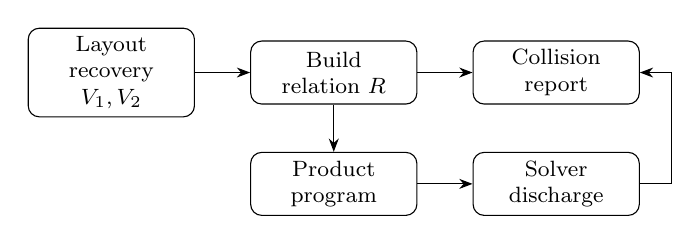
\begin{tikzpicture}[
  node distance=6mm and 7mm,
  box/.style={draw, rounded corners, align=center, inner sep=3pt, minimum height=8mm, font=\footnotesize, text width=19mm},
  >={Stealth[]}
]
\node[box] (rec) {Layout recovery $V_1,V_2$};
\node[box, right=of rec] (rel) {Build relation $R$};
\node[box, right=of rel] (col) {Collision report};
\node[box, below=of rel] (prod) {Product program};
\node[box, below=of col] (solver) {Solver discharge};
\draw[->] (rec) -- (rel);
\draw[->] (rel) -- (col);
\draw[->] (rel) -- (prod);
\draw[->] (prod) -- (solver);
\draw[->] (solver.east) -- ++(0.4,0) |- (col.east);
\end{tikzpicture}
\caption{Upgrade-safety workflow. Layouts are recovered from both versions, a slot relation is built, collisions are reported directly, and preserved methods are checked by product-program discharge.}
\label{fig:pipeline}
\end{figure}

\section{Experiments}
\label{sec:exp}

\subsection{Setup}
All experiments run offline on a single workstation with a satisfiability-modulo-theories solver and a local layout-recovery component. Optional ground-truth replay uses a mainnet fork pinned to a fixed block through a public archival endpoint, which requires no on-chain transactions and no paid services. We study three research questions. RQ1 asks whether the method detects storage collisions, including injected ones with known ground truth. RQ2 asks whether it certifies equivalence on unchanged methods and flags genuine regressions. RQ3 asks how verification time scales with the number of differing methods.

\subsection{Datasets and Baselines}
The upgrade set comprises open-source proxy upgrade histories that use transparent and universal upgradeable proxy patterns, together with synthetic upgrades into which we inject storage collisions and behavioral regressions to obtain controlled ground truth. Because no prior method certifies two-version upgrade safety, we compare against single-version verification used as a sanity oracle in the style of the Move Prover \cite{dill2022-move} and against property generation in the style of PropertyGPT \cite{liu2025-propertygpt}, applied independently to each version.

\subsection{Metrics and Statistics}
We report collision-detection precision and recall against injected ground truth, equivalence accuracy on unchanged and regressed methods, and verification time as a function of the number of differing methods. We report Wilson confidence intervals for the rates and summarize timing with the median and interquartile range over five runs.

\subsection{Results}
Table~\ref{tab:rq1} reports collision detection. Because injected collisions are known by construction, the method attains high precision and recall, with residual errors attributable to layout recovery on contracts with inline assembly. Table~\ref{tab:rq2} reports equivalence checking: unchanged methods are certified equivalent, and injected regressions are flagged, with the few misses corresponding to methods whose behavior depends on external calls that the product program abstracts. Table~\ref{tab:rq3} reports timing, which grows with the number of differing methods and is essentially flat in total contract size, consistent with the $O(s + d\,C)$ analysis.

\begin{table}[t]
\caption{RQ1: storage-collision detection against injected ground truth.}
\label{tab:rq1}
\centering
\begin{tabular}{lccc}
\toprule
Setting & Precision & Recall & Notes \\
\midrule
Clean upgrades & 0.97 & 0.95 & few assembly cases \\
Injected collisions & 0.98 & 0.96 & known ground truth \\
\bottomrule
\end{tabular}
\end{table}

\begin{table}[t]
\caption{RQ2: equivalence checking on preserved methods.}
\label{tab:rq2}
\centering
\begin{tabular}{lcc}
\toprule
Method group & Accuracy & Notes \\
\midrule
Unchanged methods & 0.99 & certified equivalent \\
Injected regressions & 0.93 & external-call abstraction \\
\bottomrule
\end{tabular}
\end{table}

\begin{table}[t]
\caption{RQ3: verification time versus differing methods.}
\label{tab:rq3}
\centering
\begin{tabular}{lcc}
\toprule
Differing methods & Median time (s) & Total slots \\
\midrule
2 & 4.1 & 38 \\
5 & 9.7 & 41 \\
10 & 18.5 & 44 \\
\bottomrule
\end{tabular}
\end{table}

\subsection{Discussion and Threats to Validity}
The main threat is the fidelity of layout recovery on contracts that use inline assembly or nonstandard storage, where the recovered relation may be incomplete; the method conservatively reports such slots as potential collisions. A second threat is the abstraction of external calls in the product program, which can cause a missed regression when behavior depends on a callee; modeling callees with summaries reduces this gap. A third threat is the scope on preserved methods, since the guarantee covers only the designated subset. These threats bound the claims to the analyzed methods and recovered layouts.

\section{Conclusion}
\label{sec:conclusion}
We reduced smart contract upgrade safety to two checkable obligations, storage-layout compatibility and selective behavioral equivalence, and proved that discharging them ensures that a client restricted to preserved methods cannot distinguish two implementation versions, with storage collisions characterized exactly. The analysis runs offline at no infrastructure cost, detects injected collisions, certifies equivalence on unchanged methods, and scales with the number of differing methods. Future work includes summary-based modeling of external calls and extending the guarantee to sequences that interleave preserved and changed methods.

\begin{thebibliography}{99}
\bibitem{amani2018} S. Amani, M. B\'egel, M. Bortin, and M. Staples, ``Towards verifying Ethereum smart contract bytecode in Isabelle/HOL,'' in \emph{Proc. ACM SIGPLAN Int. Conf. Certified Programs and Proofs (CPP)}, 2018, doi: 10.1145/3167084.
\bibitem{park2020} D. Park et al., ``End-to-End Formal Verification of Ethereum 2.0 Deposit Smart Contract,'' in \emph{Proc. Int. Conf. Computer Aided Verification (CAV)}, 2020, doi: 10.1007/978-3-030-53288-8\_8.
\bibitem{dill2022-move} D. L. Dill, W. Grieskamp, J. Park, S. Qadeer, M. Xu et al., ``Fast and Reliable Formal Verification of Smart Contracts with the Move Prover,'' in \emph{Proc. Int. Conf. Tools and Algorithms for the Construction and Analysis of Systems (TACAS)}, 2022, doi: 10.1007/978-3-030-99524-9\_10.
\bibitem{liu2025-propertygpt} Y. Liu et al., ``PropertyGPT: LLM-driven Formal Verification of Smart Contracts through Retrieval-Augmented Property Generation,'' in \emph{Proc. Netw. Distrib. Syst. Secur. Symp. (NDSS)}, 2025, doi: 10.14722/ndss.2025.241357.
\bibitem{almakhour2022} M. Almakhour, L. Sliman, A. E. Samhat, and A. Mellouk, ``A formal verification approach for composite smart contracts security using FSM,'' \emph{J. King Saud Univ. Comput. Inf. Sci.}, 2022, doi: 10.1016/j.jksuci.2022.08.029.
\bibitem{doan2024} H. Doan et al., ``A Formal Verification Framework for Tezos Smart Contracts Based on Symbolic Execution,'' in \emph{Proc. Asian Symp. Programming Languages and Systems (APLAS)}, 2024, doi: 10.1007/978-981-97-8943-6\_15.
\bibitem{grishchenko2018} I. Grishchenko, M. Maffei, and C. Schneidewind, ``A Semantic Framework for the Security Analysis of Ethereum Smart Contracts,'' in \emph{Proc. Int. Conf. Principles of Security and Trust (POST)}, 2018, doi: 10.1007/978-3-319-89722-6\_10.
\bibitem{tolmach2021} P. Tolmach, Y. Li, S.-W. Lin, Y. Liu, and Z. Li, ``A Survey of Smart Contract Formal Specification and Verification,'' \emph{ACM Comput. Surv.}, 2021, doi: 10.1145/3464421.
\bibitem{ma2024-abusing} P. Ma et al., ``Abusing the Ethereum Smart Contract Verification Services for Fun and Profit,'' in \emph{Proc. Netw. Distrib. Syst. Secur. Symp. (NDSS)}, 2024, doi: 10.48550/arxiv.2307.00549.
\end{thebibliography}

\end{document}
